\documentclass[13pt, a4paper, twoside]{article}
\usepackage[utf8]{inputenc}
\usepackage{array}
\usepackage{geometry}
\usepackage[czech]{babel}
\usepackage{chemformula}
\usepackage{chemfig}
\usepackage{enumitem}
\usepackage{fancyhdr}
\usepackage{setspace}
\usepackage{float}
\usepackage{multicol}
\geometry{legalpaper, margin=1.05in}
\pagestyle{fancy}
\lhead{\Large Šárka Doležalová, skupina 6}
\rhead{\large 4.11.2020}
\begin{document}
\begin{center}
    \huge
    Úloha 7: Stanovení Rozdělovacího koeficientu jódu
    \vspace{7mm}
\end{center}
\onehalfspacing
\large \noindent
\section*{Zadané úkoly}
Stanovení rozdělovacího koeficientu jódu ve směsi chloroform : voda a směsi toulen : voda.
\section*{Teoretický úvod}
\subsection*{Dělení nemísitelných kapalin}
Dělení nemísitelných kapalin je založeno na rozdílné hustotě dvou kapalin a dělá se s pomocí dělící nálevky. Emulzi přelijeme do dělící nálevky, kde ji ponecháme v klidu, než se kapaliny rozdělí. Poté opatrným odpouštěním kapaliny rozdělíme.
\subsection*{Titrace}
Při titraci zjišťujeme odměrné stanovení koncentrace látky v roztoku. Tuto koncentraci můžeme vyjadřovat různými veličinami, ale nejčastěji se používá molarita.(molární koncentrace, c)
\begin{align*}
    c=\frac{n}{V}
\end{align*}

Titrujeme tak, že postupně po kapkách přidáváme roztok titračního činidla z byrety do Erlenmeyerovy baňky,  ve které máme titrovanou látku. Během toho krouživým pohybem v zápěstí látku stále promícháváme. Titrační činidlo přidáváme dokud neznamenáme konec chemické reakce.
\subsection*{Distribuční koeficient}
Distribuční koeficient je veličina, která popisuje relativní afinitu dané látky ke dvěma vzájemně nemísitelným rozpouštědlům.
\begin{align*}
    K'(\frac{org. rozp.}{H_2O}) = \frac{[I_2(org. rozp.)]}{[I_2(H_2O)]}
\end{align*}
\section*{Postup}
Ve Erlenmeyerově baňce bylo v 50 ml chloroformu rozpuštěno 0,32 g jodu. Roztok byl déle přefiltrovám pomocí nálevky a kousku vaty do dělící nálevky, kam bylo přidáné i 170 ml vody. Dělící nálevka byla důkladně uzavřena a vše bylo pečlivě promícháno. 

Nálevka byla ponechána v klidu, aby se jednotlivé části oddělily. Na spodu se vytvořila vrstva chloroformu, která byla následně odpuštěna do Erlenmeyerovy baňky. Z vrchu vodné fáze bylo odpipetováno 50 ml a poté přeneseno do titrační baňky, dále bylo přidáno 10 ml zředěné HCl (1:1) a 0,5 g KI. Roztok byl titrován odměrným roztokem thiosíranu (c = 0,002 M) do zesvětlení žlutého zbarvení. Poté byl injekční stříkačkou přidán škrobový maz a roztok byl dotitrován do úplného odbarvení. Pro přesnost výsledků bylo vše zopakováno.
Malou stříkačkou byl do titrační baňky odměřen 1 ml chloroformové fáze, 50 ml destilované vody, 10 ml zředěné HCl (1:1) a přidáno 0,5 KI. Roztok byl titrován stejně až do úplného odbarvení. A poté pro správnost opět zopakován.

Z průměrné spotřeby byla vypočtena koncentrace jódu ve vodní a chloroformové fázi z toho byl spočítán distribuční koeficient.
Celý proces byl zopakován i s emulzí obsahující toluen.

\begin{figure}[H]
    \centering
    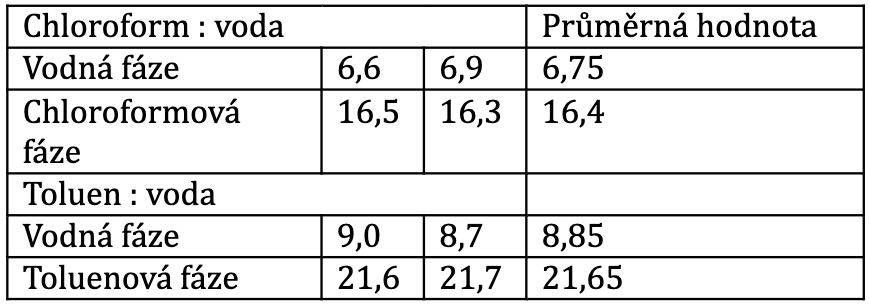
\includegraphics[width=13cm]{hh.png}
\end{figure}

\section*{Výpočet}
\subsection*{Stanovení distribučního koeficientu jódu ve směsi chloroform : voda}
\begin{align*}
    c_{S_2O_3^{2-}} = 0,002\: mol \cdot dm^{-3}
\end{align*}
\subsubsection*{Chloroform}
\begin{align*}
    c_{I_2, CHCl_3} &= c_{S_2O_3^{2-}} \cdot \frac{V_{S_2O_3^{2-}}}{2} \cdot V_{I_2, CHCl_3}\\
    c_{I_2, CHCl_3} &= 1,64 \cdot 10^{-2}\: g \cdot dm^{-3}
\end{align*}

\subsubsection*{Voda}
\begin{align*}
    c_{I_2, H_2O} &= c_{S_2O_3^{2-}} \cdot c_{S_2O_3^{2-}} \cdot \frac{V_{S_2O_3^{2-}}}{2} \cdot V_{I_2, H_2O}\\
    c_{I_2, H_2O} &= 1,35 \cdot 10^{-4} \: g\cdot dm^{-3}
\end{align*}

\subsubsection*{Koeficient}
\begin{align*}
    K' &= \frac{c_{I_2, CHCl_3}}{c_{I_2, H_2O}}\\
    K' &= 122
\end{align*}

\subsection*{Stanovení distribučního koeficientu jódu ve směsi toulen : voda}
\begin{align*}
    c_{S_2O_3^{2-}} = 0,002\: mol \cdot dm^{-3}
\end{align*}
\subsubsection*{Toulen}
\begin{align*}
    c_{I_2, H_2O} &= c_{S_2O_3^{2-}} \cdot c_{S_2O_3^{2-}} \cdot \frac{V_{S_2O_3^{2-}}}{2} \cdot V_{I_2, toulen}\\
    c_{I_2, H_2O} &= 2,165 \cdot 10^{-2} \: g\cdot dm^{-3}
\end{align*}

\subsubsection*{Voda}
\begin{align*}
    c_{I_2, H_2O} &= c_{S_2O_3^{2-}} \cdot c_{S_2O_3^{2-}} \cdot \frac{V_{S_2O_3^{2-}}}{2} \cdot V_{I_2, H_2O}\\
    c_{I_2, H_2O} &= 1,77 \cdot 10^{-4} \: g\cdot dm^{-3}
\end{align*}

\subsubsection*{Koeficient}
\begin{align*}
    K' &= \frac{c_{I_2, toulen}}{c_{I_2, H_2O}}\\
    K' &= 189
\end{align*}

\section*{Závěr}
Distribuční koeficient jodu s chloroformem a vodou jsem vypočítala na 122 a u toluenu a vody na 189. Moje výsledky je odlišují od tabulkových hodnot, ale to může být způsobeno nepřesným titrováním.


\end{document}